% paper/sections/casestudy4.tex — Case Study 4: Berkeley growth (composable sklearn Pipeline + nested GridSearchCV)
% Every number below is a macro written by paper/code/casestudy4.py into
% sections/cs4_numbers.tex (drift gate: paper/code/check_cs_numbers.py).
% Auto-generated by paper/code/casestudy4.py -- do not edit.
% Regenerate: PYTHONPATH=scripts:paper/code python paper/code/casestudy4.py
% Drift gate: PYTHONPATH=scripts:paper/code python paper/code/check_cs_numbers.py
\newcommand{\csFourNChildren}{93}
\newcommand{\csFourNBoys}{39}
\newcommand{\csFourNGirls}{54}
\newcommand{\csFourNAges}{31}
\newcommand{\csFourAgeMin}{1}
\newcommand{\csFourAgeMax}{18}
\newcommand{\csFourGrid}{2, 3, 4, 6}
\newcommand{\csFourNInner}{5}
\newcommand{\csFourNOuter}{5}
\newcommand{\csFourNRep}{10}
\newcommand{\csFourNOuterFolds}{50}
\newcommand{\csFourHeightTwo}{0.967}
\newcommand{\csFourHeightThree}{0.957}
\newcommand{\csFourHeightFour}{0.957}
\newcommand{\csFourHeightSix}{0.967}
\newcommand{\csFourVelocityTwo}{0.894}
\newcommand{\csFourVelocityThree}{0.882}
\newcommand{\csFourVelocityFour}{0.925}
\newcommand{\csFourVelocitySix}{0.957}
\newcommand{\csFourBestRep}{height}
\newcommand{\csFourBestK}{2}
\newcommand{\csFourBestKWord}{two}
\newcommand{\csFourNested}{0.970}
\newcommand{\csFourNestedSd}{0.036}
\newcommand{\csFourBaseEighteen}{0.862}
\newcommand{\csFourBaseEighteenSd}{0.058}
\newcommand{\csFourBaseTwo}{0.962}
\newcommand{\csFourBaseTwoSd}{0.043}
\newcommand{\csFourAgeEarly}{12}


\subsection{Composable scikit-learn Pipelines: Berkeley Growth Data}
\label{subsec:cs4-growth}

This study showcases the \emph{composability} of the \texttt{fdars}
scikit-learn layer on a genuinely functional problem: predicting a child's sex
from their growth curve.  The Berkeley growth study
\citep{tuddenham_snyder_1954}, in the version distributed with the R
\texttt{fda} package \citep{r_fda} and analysed by
\citet{ramsay_silverman_2005}, records the heights of
\csFourNChildren{} children (\csFourNBoys{} boys, \csFourNGirls{} girls) at
\csFourNAges{} ages between \csFourAgeMin{} and \csFourAgeMax{} years.  Adult height alone separates the
sexes only partly; the timing of the pubertal growth spurt---earlier in
girls---carries additional information that a curve-level method can use.

\paragraph{Pipeline and search.}
The pipeline chains three steps: an optional representation step (either the
height curves themselves or growth-velocity curves, obtained by GCV B-spline
smoothing and differentiation with \texttt{fdars} functions wrapped in a
scikit-learn \texttt{FunctionTransformer}), an \texttt{fdars}
\texttt{FPCATransformer}, and scikit-learn's own
\texttt{LinearDiscriminantAnalysis}.  \texttt{GridSearchCV} treats the
representation as an ordinary hyperparameter alongside the number of FPCA
components, $\{\csFourGrid\}$, using seeded stratified \csFourNInner-fold
cross-validation.  No adapter code is needed: every step obeys the
scikit-learn estimator contract.

\paragraph{Results.}
Height curves score higher than velocity curves at every dimension
(Figure~\ref{fig:cs4-gridsearch}; mean inner CV accuracy $\csFourHeightTwo$, $\csFourHeightThree$,
$\csFourHeightFour$, $\csFourHeightSix$ for $\csFourGrid$ components, against
$\csFourVelocityTwo$, $\csFourVelocityThree$, $\csFourVelocityFour$,
$\csFourVelocitySix$ for velocity), and the search selects \csFourBestRep{}
curves with \csFourBestKWord{} components\csFourBestTie{}.  Because a score used for selection is optimistically biased, we
evaluate the \emph{entire} search by nested cross-validation (an outer
stratified \csFourNOuter-fold split repeated \csFourNRep{} times).  Because the
inner search may choose different configurations in different outer folds,
this scores the complete selection procedure rather than one fixed pipeline:
it attains a mean accuracy of $\csFourNested$ (standard deviation
$\csFourNestedSd$ across the \csFourNOuterFolds{} outer folds).  Under the
identical outer splits, a logistic regression on final height alone reaches
$\csFourBaseEighteen$ (s.d.\ $\csFourBaseEighteenSd$), and one on the heights at
ages \csFourAgeEarly{} and \csFourAgeMax---an expert's hand-picked
``before and after puberty'' pair---reaches $\csFourBaseTwo$
(s.d.\ $\csFourBaseTwoSd$).  The functional
pipeline thus matches the expert feature choice without being told which ages
matter.  Figure~\ref{fig:cs4-scores} shows why \csFourBestKWord{} components suffice: the
first is an overall size mode and the second a growth-timing mode (compare
Figure~\ref{fig:tour-fpca}), and together they separate boys from girls
almost linearly.
The analysis is reproduced by \texttt{paper/code/casestudy4.py}.

\begin{figure}[tbp]
  \centering
  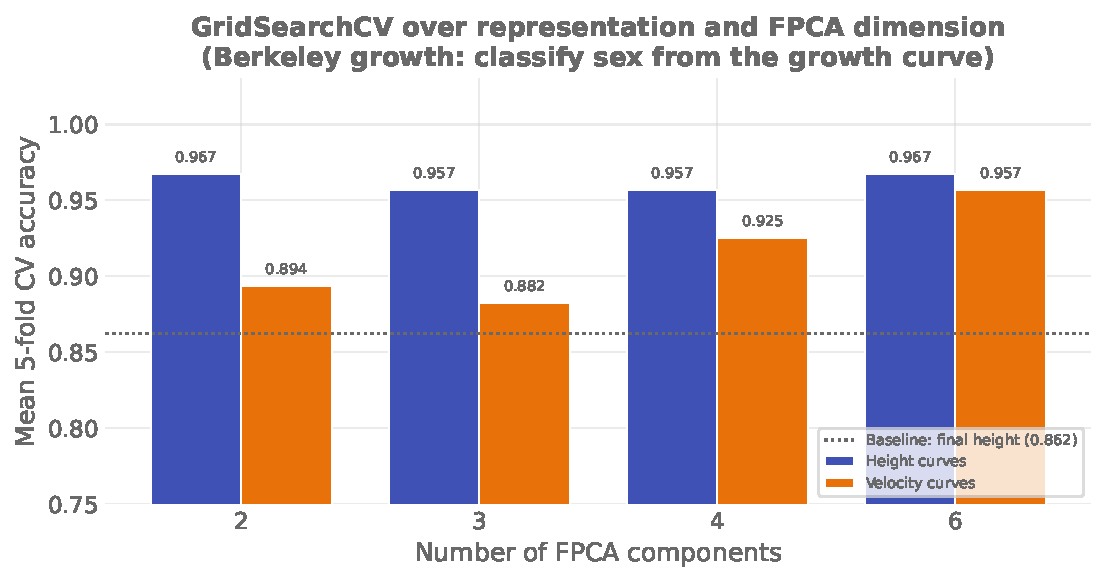
\includegraphics[width=\textwidth]{figures/cs4_growth_gridsearch.pdf}
  \caption{\texttt{GridSearchCV} over the functional representation (height
    or velocity curves) and the number of FPCA components, for the pipeline
    representation $\to$ \texttt{FPCATransformer} $\to$
    \texttt{LinearDiscriminantAnalysis}.  Bars show the mean inner
    \csFourNInner-fold CV accuracy of the grid search (one seeded split of the
    full sample); the dotted line is a logistic regression on final height
    alone, scored by the repeated (\csFourNRep$\times$\csFourNOuter-fold) outer
    CV, so the two are not scored on identical splits.}
  \label{fig:cs4-gridsearch}
\end{figure}

\begin{figure}[tbp]
  \centering
  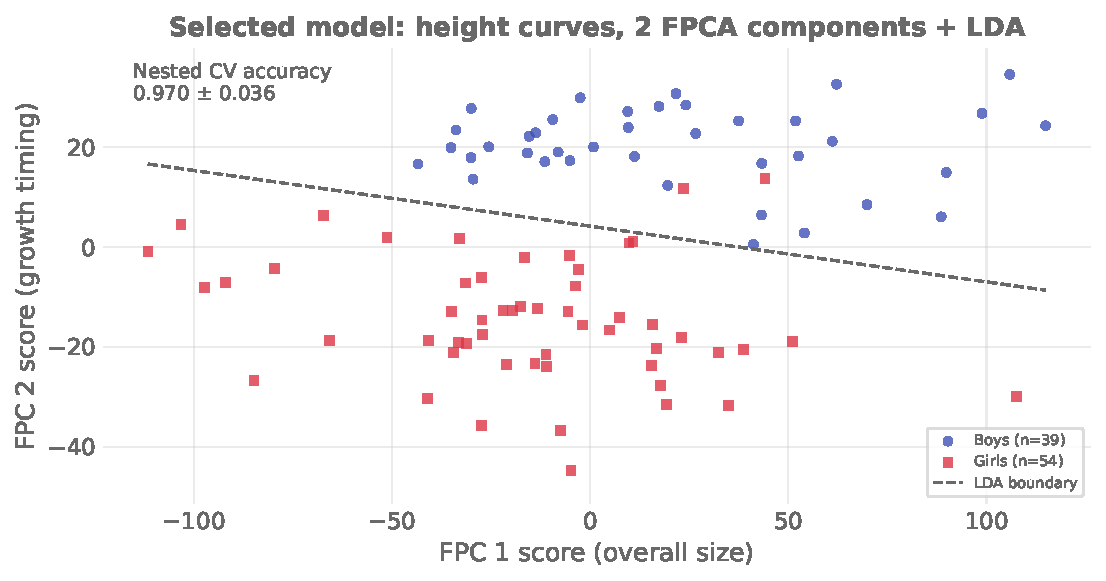
\includegraphics[width=\textwidth]{figures/cs4_growth_scores.pdf}
  \caption{FPCA scores of the selected model (\csFourBestRep{} curves,
    \csFourBestKWord{} components),
    coloured by sex, with the LDA decision boundary.  The first component
    reflects overall size and the second the timing of the growth spurt; the
    box reports the nested cross-validated accuracy of the whole search (mean
    $\pm$ standard deviation over the \csFourNOuterFolds{} outer folds).}
  \label{fig:cs4-scores}
\end{figure}
